\documentclass[tikz,border=10pt]{standalone}
\usetikzlibrary{calc}
\begin{document}
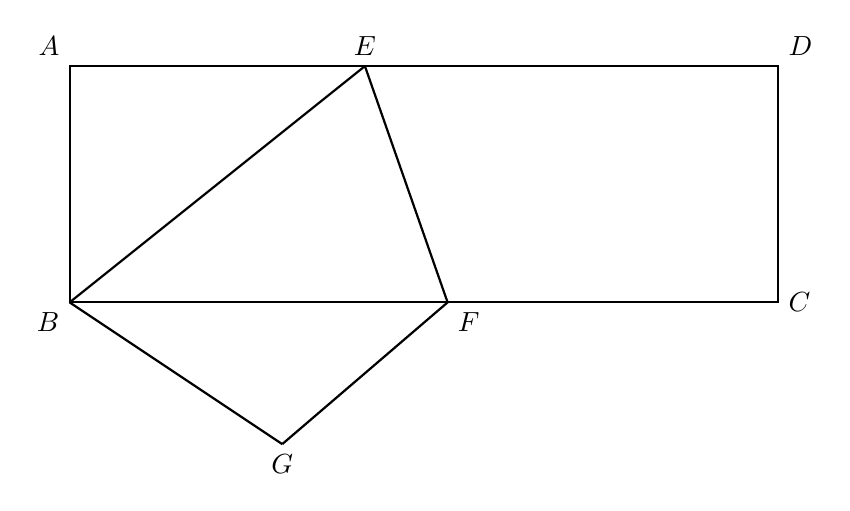
\begin{tikzpicture}[thick, scale=1.5]    
% 1. 定义坐标 (矩形宽高设定为 4x2)    
\coordinate (B) at (-1,0);    
\coordinate (A) at (-1,2);    
\coordinate (D) at (5,2);    
\coordinate (C) at (5,0);        
% 定义 E 为 AD 上的点, F 为 BC 上的点    
\coordinate (E) at (1.5, 2);    
\coordinate (F) at (2.2, 0);        
% 计算 G 的位置 (基于视觉参考)    
\coordinate (G) at (0.8, -1.2);
    % 2. 绘制矩形边界    
\draw (A) -- (D) -- (C) -- (B) -- cycle;
    % 3. 绘制内部连线    
\draw (B) -- (E); % 线段 BE    
\draw (E) -- (F); % 线段 EF    
\draw (B) -- (G); % 线段 BG    
\draw (F) -- (G); % 线段 FG        
% 4. 标注顶尖 (Label)    
\node[above left] at (A) {$A$};    
\node[below left] at (B) {$B$};    
\node[above]     at (E) {$E$};    
\node[below right] at (F) {$F$};    
\node[right]     at (C) {$C$};    
\node[above right] at (D) {$D$};    
\node[below]     at (G) {$G$};
\end{tikzpicture}
\end{document}